\documentclass[12pt]{article}
\usepackage[margin=2.5cm]{geometry}
\usepackage{enumerate}
\usepackage{amsfonts}
\usepackage{amsmath}
\usepackage{fancyhdr}
\usepackage{amsmath}
\usepackage{amssymb}
\usepackage{amsthm}
\usepackage{mdframed}
\usepackage{graphicx}
\usepackage{subcaption}
\usepackage{adjustbox}
\usepackage{listings}
\usepackage{xcolor}
\usepackage{booktabs}
\usepackage[utf]{kotex}
\usepackage{hyperref}

\definecolor{codegreen}{rgb}{0,0.6,0}
\definecolor{codegray}{rgb}{0.5,0.5,0.5}
\definecolor{codepurple}{rgb}{0.58,0,0.82}
\definecolor{backcolour}{rgb}{0.95,0.95,0.92}

\lstdefinestyle{mystyle}{
    backgroundcolor=\color{backcolour},
    commentstyle=\color{codegreen},
    keywordstyle=\color{magenta},
    numberstyle=\tiny\color{codegray},
    stringstyle=\color{codepurple},
    basicstyle=\ttfamily\footnotesize,
    breakatwhitespace=false,
    breaklines=true,
    captionpos=b,
    keepspaces=true,
    numbers=left,
    numbersep=5pt,
    showspaces=false,
    showstringspaces=false,
    showtabs=false,
    tabsize=1
}

\lstset{style=mystyle}

\pagestyle{fancy}
\renewcommand{\headrulewidth}{0.4pt}
\lhead{Team Treehouse}
\rhead{Java Objects Part 3 Notes}

\begin{document}
\title{Java Objects Part 3 Notes}
\author{Team Treehouse}
\maketitle

\section{Planning the MVP}

\begin{itemize}

    \item Priortized backlog of user stories $\Rightarrow$ a common way of handling scope
    \begin{itemize}
        \item Uses Kanban board

        \begin{center}
        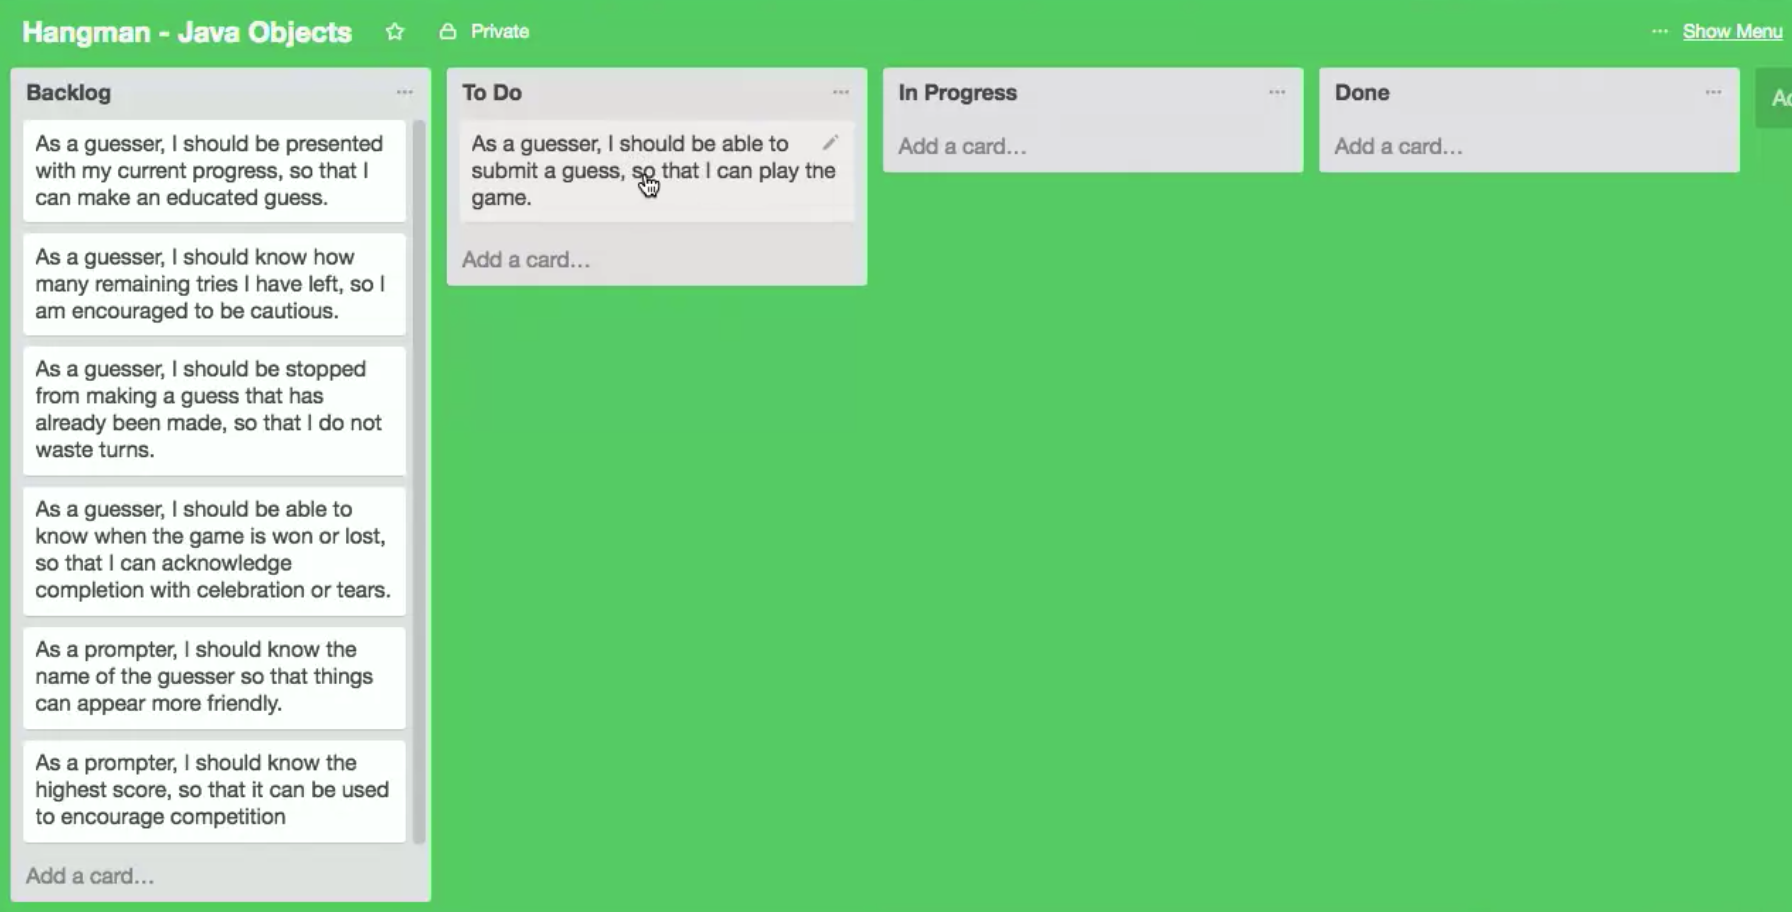
\includegraphics[width=\linewidth]{images/part_3_notes_1.png}
        \end{center}
    \end{itemize}

    \item Common format of a user story
    \begin{center}
    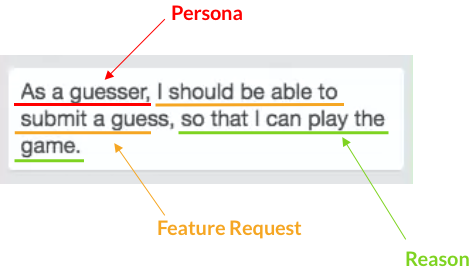
\includegraphics[width=0.65\linewidth]{images/part_3_notes_2.png}
    \end{center}
    \item Sprint $\Rightarrow$ Set period of time a list during which work
    will be completed and will be ready for review (i.e. By the end of the day,
    dun dun dun...)

    \begin{center}
    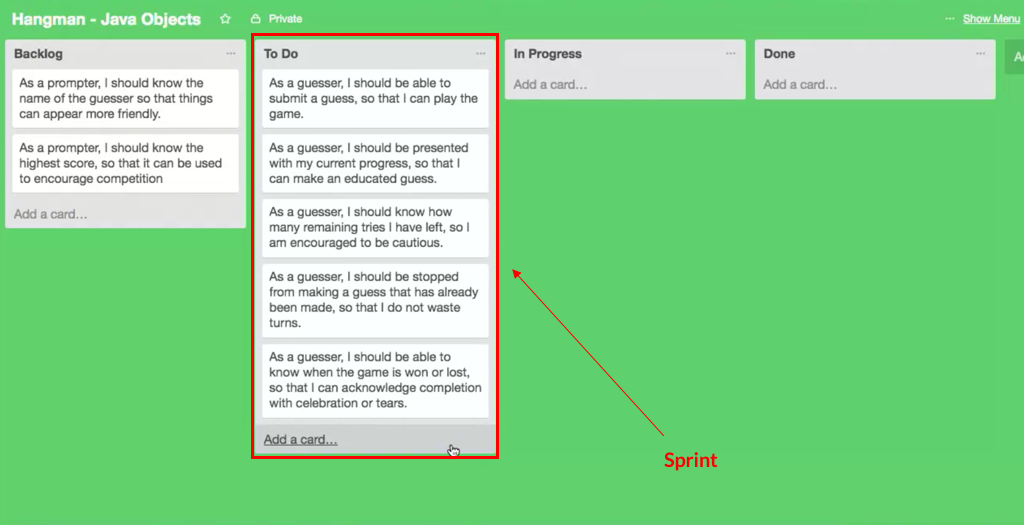
\includegraphics[width=\linewidth]{images/part_3_notes_3.png}
    \end{center}
\end{itemize}

\bigskip

\section{Quiz 1}

\bigskip

\begin{enumerate}[1.]
    \item

    The set of software development practices we talked about exploring is called

    \bigskip

    \begin{enumerate}[A.]
        \item CS
        \item Bubble Sort
        \item Agile
        \item Brogramming
    \end{enumerate}

    \bigskip

    \textbf{Answer:} C

    \item

    An MVP can be created by

    \bigskip

    \begin{enumerate}[A.]
        \item defining the minimum requirements to prove that the product is working as hypothesized.
        \item taking existing code and refactoring it so it is smaller and more compact
        \item minimizing the number of people working on the project so that the knowledge is with one person only
        \item coming up with every possible roadblock and feature that might occur and map it out on a Gantt chart
    \end{enumerate}

    \bigskip

    \textbf{Answer:} A

    \item

    An MVP in our context stands for

    \bigskip

    \begin{enumerate}[A.]
        \item Mostly Verbatim Process
        \item Most Valuable Player
        \item Minimum Viable Product
    \end{enumerate}

    \bigskip

    \textbf{Answer:} C

\end{enumerate}

\bigskip

\section{Getting Started}

\bigskip

\begin{itemize}
    \item Separation of concerns heavily considered
    \begin{itemize}
        \item The Goal is to make the code as reusable as possible, i.e. The same game
        logic should be applicable in desktop, website, phone in medium other than
        console

        \begin{center}
        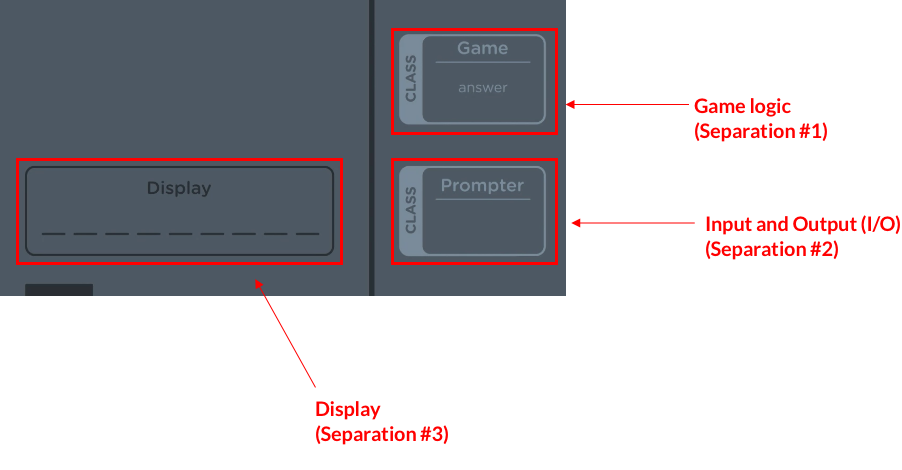
\includegraphics[width=\linewidth]{images/part_3_notes_4.png}
        \end{center}

    \end{itemize}

    \begin{lstlisting}[language=Java,caption={lesson\_03/Game.java}]
    public class Game {
        private String answer;

        public Game(String answer) {
            this.answer = answer;
        }
    }
    \end{lstlisting}

    \begin{lstlisting}[language=Java,caption={lesson\_03/Hangman.java}]
    public class Hangman {

        public static void main(string[] args) {
            Game game = new Game("treehouse");
        }

    }
    \end{lstlisting}
\end{itemize}
\bigskip

\section{Quiz 1}

\bigskip

\begin{enumerate}[1.]
    \item

    What concerns have we chosen to separate?

    \bigskip

    \begin{enumerate}[A.]
        \item We are separating the answer from the guesser.
        \item We have chosen to separate the display of the game from the logic, or state, of the game.
        \item We are separating letters from each other so that we can make spaces.
    \end{enumerate}

    \bigskip

    \textbf{Answer:} B

    \item

    Due to the separation we have chosen, what outcome can we expect?

    \bigskip

    \begin{enumerate}[A.]
        \item We will be able to run this in other languages like JavaScript or Python.
        \item We can more easily generate code using external tools.
        \item We will be able to use the same game logic in other applications, such as console applications, web sites and apps.
    \end{enumerate}

    \bigskip

    \textbf{Answer:} C

\end{enumerate}

\bigskip

\section{Storing Guesses}

\bigskip

\begin{itemize}
    \item \textit{STRING\_VAR.indexOf(VAL)}: tells the index of beginning value
    of \textit{VAL} in string
\end{itemize}

    \begin{lstlisting}[language=Java,caption={lesson\_05/Game.java}]
    public class Game {
        private String answer;
        private String hits;
        private String misses;

        public Game(String answer) {
            this.answer = answer;
            this.hits = "";
            this.misses = "";
        }

        public boolean applyGuess(char letter) {
            boolean isHit = answer.indexOf(letter) != -1; // <- this guy here :)
            if (isHit) {
                hits += letter;
            } else {
                misses += letter;
            }

            return isHit;
        }
    }
    \end{lstlisting}

\bigskip

\section{Exercise 1}

\bigskip

\begin{itemize}
    \item Solution included in \textit{exercise\_1.java}
\end{itemize}

\bigskip

\section{Prompting for Guesses}

\bigskip

\begin{itemize}
    \item \textit{Scanner}
    \begin{itemize}
        \item Is similar to \textit{stdin} in \textit{C}
        \item Lives in \textit{java.util} package

    \begin{lstlisting}[language=Java,caption={lesson\_07/Prompter.java}]
    import java.util.Scanner;

    public class Prompter {
        ...

        public boolean promptForGuess() {
            Scanner scanner = new Scanner(System.in); // <- This little guy here :)
            ...
        }
    }
    \end{lstlisting}

    \end{itemize}
\end{itemize}

\end{document}